% This file was created with tikzplotlib v0.10.1.
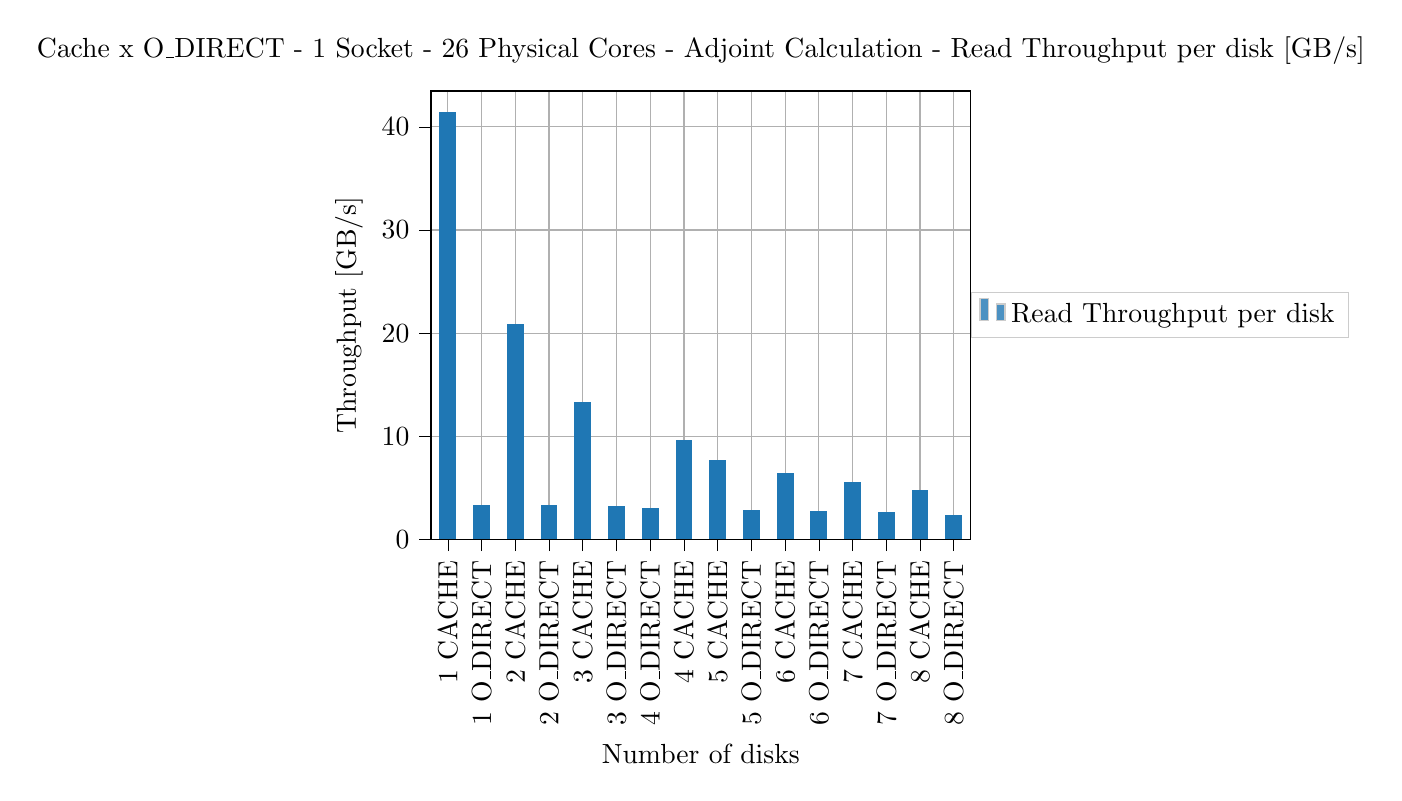
\begin{tikzpicture}

\definecolor{darkgray176}{RGB}{176,176,176}
\definecolor{lightgray204}{RGB}{204,204,204}
\definecolor{steelblue31119180}{RGB}{31,119,180}

\begin{axis}[
legend cell align={left},
legend style={
  fill opacity=0.8,
  draw opacity=1,
  text opacity=1,
  at={(1,0.5)},
  anchor=west,
  draw=lightgray204
},
tick align=outside,
tick pos=left,
title={Cache x O\_DIRECT - 1 Socket - 26 Physical Cores - Adjoint Calculation - Read Throughput per disk [GB/s]},
x grid style={darkgray176},
xlabel={Number of disks},
xmajorgrids,
xmin=-0.5, xmax=15.5,
xtick style={color=black},
xtick={0,1,2,3,4,5,6,7,8,9,10,11,12,13,14,15},
xticklabel style={rotate=90.0},
xticklabels={
  1 CACHE,
  1 O\_DIRECT,
  2 CACHE,
  2 O\_DIRECT,
  3 CACHE,
  3 O\_DIRECT,
  4 O\_DIRECT,
  4 CACHE,
  5 CACHE,
  5 O\_DIRECT,
  6 CACHE,
  6 O\_DIRECT,
  7 CACHE,
  7 O\_DIRECT,
  8 CACHE,
  8 O\_DIRECT
},
y grid style={darkgray176},
ylabel={Throughput [GB/s]},
ymajorgrids,
ymin=0, ymax=43.4911282688394,
ytick style={color=black}
]
\draw[draw=none,fill=steelblue31119180] (axis cs:-0.25,0) rectangle (axis cs:0.25,41.4201221607994);
\addlegendimage{ybar,ybar legend,draw=none,fill=steelblue31119180}
\addlegendentry{Read Throughput per disk}

\draw[draw=none,fill=steelblue31119180] (axis cs:0.75,0) rectangle (axis cs:1.25,3.30335186239196);
\draw[draw=none,fill=steelblue31119180] (axis cs:1.75,0) rectangle (axis cs:2.25,20.9190912);
\draw[draw=none,fill=steelblue31119180] (axis cs:2.75,0) rectangle (axis cs:3.25,3.32844835893762);
\draw[draw=none,fill=steelblue31119180] (axis cs:3.75,0) rectangle (axis cs:4.25,13.2858922414201);
\draw[draw=none,fill=steelblue31119180] (axis cs:4.75,0) rectangle (axis cs:5.25,3.18484509049645);
\draw[draw=none,fill=steelblue31119180] (axis cs:5.75,0) rectangle (axis cs:6.25,3.057624769133);
\draw[draw=none,fill=steelblue31119180] (axis cs:6.75,0) rectangle (axis cs:7.25,9.59536661880342);
\draw[draw=none,fill=steelblue31119180] (axis cs:7.75,0) rectangle (axis cs:8.25,7.70923875982833);
\draw[draw=none,fill=steelblue31119180] (axis cs:8.75,0) rectangle (axis cs:9.25,2.82429658968554);
\draw[draw=none,fill=steelblue31119180] (axis cs:9.75,0) rectangle (axis cs:10.25,6.42896432011453);
\draw[draw=none,fill=steelblue31119180] (axis cs:10.75,0) rectangle (axis cs:11.25,2.6978861986182);
\draw[draw=none,fill=steelblue31119180] (axis cs:11.75,0) rectangle (axis cs:12.25,5.51448822464183);
\draw[draw=none,fill=steelblue31119180] (axis cs:12.75,0) rectangle (axis cs:13.25,2.62290479100511);
\draw[draw=none,fill=steelblue31119180] (axis cs:13.75,0) rectangle (axis cs:14.25,4.8182742248927);
\draw[draw=none,fill=steelblue31119180] (axis cs:14.75,0) rectangle (axis cs:15.25,2.31555426827088);
\end{axis}

\end{tikzpicture}
